\documentclass{swp1}
\usepackage[utf8]{inputenc}
\usepackage{amssymb}
\usepackage{url}


% Tabellen
\usepackage{tabularx}
\usepackage{supertabular}
\usepackage{booktabs}







\begin{document}

% \maketitle{Nummer}{Abgabedatum}{Tutor-Name}{Gruppennummer}
%           {Teilnehmer 1}{Teilnehmer 2}{Teilnehmer 3}
\maketitle{3}{29.06.2014}{Michaela Bunke}{ChronoX}
          {Tim Ellhoff}{Karsten Betjemann}{}
          
\section*{Aufgabe 1)}

Der Anwendungsfall dieser Aufgabe lässt sich am einfachsten anhand des zentralen Prozesses \textit{Einschreibung an der Universität} beschreiben.\newline
In Bezug auf diesen Anwendungsfall gibt es drei interagierende Akteure zu benennen, wobei mit \textit{StudentIn} und \textit{SachbearbeiterIn} die beiden grundsätzlich am Prozess beteiligten Akteure gelistet sind und es als eine spezifische Untergruppe von \textit{StudentIn} auch noch die Variation \textit{InternationaleR StudentIn} gibt.\newline
Der Prozess selbst wird unter der Bedingung eingeleitet, dass von Seiten eines Studenten Interesse an der Einschreibung an der Universität besteht, sowie, dass eine Sachbearbeiterin zur Bearbeitung der Aufgabe zur Verfügung steht und auf sämtliche notwendigen Systeme und Daten zugreifen kann.\newline
Beim eigentlichen Prozessablauf tätigen Mitarbeiter und Student die Einschreibung dergestalt gemeinsam, als dass die für die Einschreibung nötigen Informationen vom Studenten an die Mitarbeiterin ausgegeben werden, die die Einschreibung vornimmt. Zuletzt kann auch eine \textit{Einschreibung für einen Studiengang} durchgeführt werden, auch wenn dies nicht notwendigerweise Teil des Prozessablaufs sein muss. Die Einschreibung für ein \textit{Studium Generale} steht in einer Vererbungsbeziehung zur \textit{Einschreibung an der Universität} und in dieser Hinsicht in Beziehung zu diesem Prozessablauf.\newline
Die nennenswerte Variation im Prozessablauf basiert auf der Vorbedingung, dass der Akteur \textit{StudentIn} der Gruppe \textit{InternationaleR StudentIn} zugeordnet ist. In diesem Falle kann von jener Seite aus zuvor eine \textit{Stellungnahme} des \textit{International Office} als zusätzlich für den Prozess anwendbarer Datensatz eingeholt werden.

\section*{Aufgabe 2)}

Zur Auswertung der in der Aufgabe gelisteten Szenarien bietet sich ein Vorgehen nach dem Schema der klassischen textuellen Beschreibung von Anwendungsfällen an, wobei einleitend gesagt sei, dass die in den Szenarien gelisteten Nutzfälle der Informationssuche durch Privatkunden und Großkunden, sowie der Händlerbestellung und Direktbestellung entsprechen, wobei als beteiligte Akteure Privatkunde, Großkunde, Händler und Disponent zu listen sind.\newline
\newline
\emph{Szenario 1}\newline
\textbf{Name:}\newline
Informationszugriff und Konfiguration - Privatkunde\newline
\textbf{Akteure:}\newline
Privatkunde\newline
\textbf{Vorbedingung:}\newline
Privatkunde wünscht Informationen zu spezifischem Produkt\newline
Privatkunde hat Zugang zum Informationssystem\newline
Informationssystem ist einsetzbar/verfügbar\newline
\textbf{Nachbedingung:}\newline
Privatkunde hat eigene Produktkonfiguration erstellt\newline
\textbf{Ablauf:}\newline
Privatkunde greift auf das Informationssystem zu\newline
Privatkunde sucht nach dem Modell X123\newline
Informationssystem zeigt Kenndaten von Modell X123 an\newline
Privatkunde konfiguriert Kenndaten im Sinne eines Wunschmodells\newline
\newline
\emph{Szenario 2}\newline
\textbf{Name:}\newline
Informationszugriff - Großkunde\newline
\textbf{Akteure:}\newline
Großkunde\newline
\textbf{Vorbedingung:}\newline
Großkunde wünscht Informationen über spezifisches Modell\newline
Großkunde hat Zugang zum Informationssystem\newline
Informationssystem ist einsetzbar/verfügbar\newline
\textbf{Nachbedingung:}\newline
Keine Nachbedingung\newline
\textbf{Ablauf:}\newline
Großkunde greift auf das Informationssystem zu\newline
Großkunde sucht nach dem Modell X987\newline
Informationssystem zeigt Kenndaten von Modell X987 an\newline
Großkunde sucht nach dem Modell X567\newline
Informationssystem zeigt Kenndaten von Modell X567 an\newline
Großkunde beendet das Informationssystem\newline
\newline
\emph{Szenario 3}\newline
\textbf{Name:}\newline
Händlerbestellung - Privatkunde\newline
\textbf{Akteure:}\newline
Privatkunde\newline
Händler\newline
Disponent\newline
\textbf{Vorbedingung:}\newline
Privatkunde möchte ein Modell bestellen\newline
Händler ist verfügbar\newline
Disponent ist verfügbar\newline
Informationssystem/Bestellsystem ist verfügbar\newline
Produktionssystem ist verfügbar\newline
\textbf{Nachbedingung:}\newline
Bestellung ist abgeschlossen\newline
Produktionsauftrag ist erstellt\newline
\textbf{Ablauf:}\newline
Privatkunde sucht Händler auf\newline
Händler erhält Bestelldaten von Privatkunde\newline
Händler ruft Informationssystem/Bestellsystem auf\newline
Händler sucht nach Modell X234\newline
Informationssystem/Bestellsystem zeigt Datenblatt zu Modell X234 an\newline
Händler konfiguriert das Modell nach den Wunschdaten des Kunden\newline
Händler nutzt integriert Bestellfunktion zur Bestellung von Modell X234\newline
Informationssystem/Bestellsystem leitet Bestellauftrag an Disponenten weiter\newline
Disponent bestätigt Bestellung und schließt damit die Bestellung ab\newline
Händler beendet Informationssystem/Bestellsystem\newline
Disponent ruft Produktionssystem auf\newline
Disponent erstellt Produktionsauftrag\newline
Disponent beendet Produktionssystem\newline
\newline
\emph{Szenario 4}\newline
\textbf{Name:}\newline
Direktbestellung - Großkunde\newline
\textbf{Akteure:}\newline
Großkunde\newline
Händler\newline
Disponent\newline
\textbf{Vorbedingung:}\newline
Großkunde möchte ein Modell bestellen\newline
Alle haben Zugriff auf das Informationssystem/Bestellsystem\newline
Informationssystem/Bestellsystem ist verfügbar\newline
Disponent hat Zugriff auf Produktionssystem\newline
Produktionssystem ist verfügbar\newline
\textbf{Nachbedingung:}\newline
Bestellung ist abgeschlossen\newline
Produktionsauftrag ist erstellt\newline
\textbf{Ablauf:}\newline
Großkunde ruft Informationssystem/Bestellsystem auf\newline
Großkunde sucht nach Wunschmodell\newline
System zeigt Datenblatt an\newline
Großkunde konfiguriert die Modelldaten nach Wunsch\newline
Großkunde gibt Bestellung auf\newline
Händler und Disponent bestätigen Bestellung\newline
Disponent ruft Produktionssystem auf\newline
Disponent gibt Produktiuonsauftrag aus\newline
\newline
Alle Szenarien lassen sich einem Anwendungsfalldiagramm darstellen, um den Prozessablauf schematisch zu überblicken und zu verdeutlichen.\newline
\newline
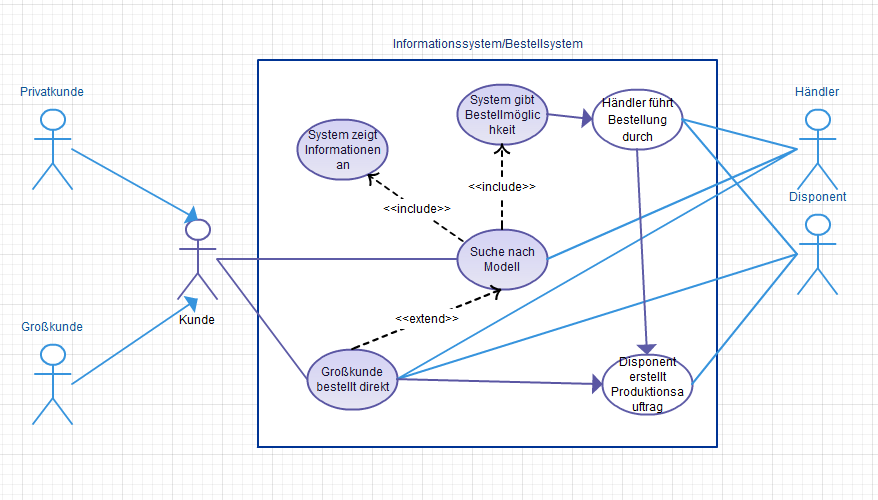
\includegraphics[scale=0.75]{Diagramm}
\newline

\section*{Aufgabe 3)}

\textbf{Assoziation:}\newline
Assoziationen sind eine Relation, welche in UML Klassendiagrammen angewandt wird, um eine Beziehung zwischen mehreren Objektinstanzen anzuzeigen.
Besondere Bedeutung hat hierbei der Umstand, dass diese Assoziationen auch eine Navigierbarkeit implizieren können, was gestalterisch durch Pfeile anzeigbar ist.\newline
Diese Navigierbarkeit ist notwendig, um im Rahmen der Implementierung erkennen zu können, ob irgendwo ein Wechsel vom einem Objekt zum anderen realisiert werden muss und ist zum Beispiel durch die Speicherung einer Objektreferenz in einem Attribut umsetzbar.\newline
\textbf{Aggregation:}\newline
Die Aggregation kann als speziellere Form der Assoziation verstanden werden, welche dazu dient, eine vereinigende Beziehung von einzelnen Objekten in einem Aggregat zu symbolisieren.
Durch diese Maßnahme lassen sich also übergeordnete Aggregate aus unterschiedlich vielen Objekten bilden, um so eine bessere Ordnung oder eine genauere Spezifikation zu ermöglichen.\newline
Eine beispielhafte Möglichkeit hierfür wäre die Unterordnung verschiedener Bücher in eine Buchreihe.\newline
\textbf{Komposition:}\newline
Die Komposition lässt sich leicht als erweiterte und stärkere Form der Aggregation verstehen, wobei hier signalisiert wird, dass das Aggregat und seine Komponenten derartig logisch miteinander verbunden sind, als dass die Komponenten selbst nicht ohne das Aggregat vorhanden sein können. Es existiert also eine ständige und starke Bindung zwischen beiden. Diese beruht auch darauf, dass eine Komposition nur zwischen den Komponenten und jeweils einem Aggregat bestehen kann.\newline
Als logisches Beispiel könnte man eine Buchreihe durch Komposition mit einem Verlag darstellen, um zu signalisieren, dass eine Buchreihe nicht ohne den dazugehörigen Verlag existieren kann, auch wenn dieses Beispiel im Zusammenhang mit der modernen Eigenpublikation vielleicht an Schärfe verlieren kann.\newline
\textbf{Generalisierung:}\newline
Generalisierungen sind eine praktische Relation zur Umsetzung von Vererbungshierarchien auf der schematischen Ebene von oberen und unteren Klassen. Sie kennzeichnen voneinander erbende Klassen und geben gleichzeitig die Richtung in der Erbhierarchie an, wobei die unteren Klassen die Attribute und Methoden der oberen Klassen erben, selbige aber auch beliebig umschreiben und erweitern oder aber auch neue Methoden und Attribute definieren können. Im Rahmen der Generalisierungen können auch abstrakte Klassen angelegt werden, die nur zur Einfachheit mehrere Eigenschaften vererbbar in sich vereinigen, als Objekt angewandt jedoch nicht vorkommen.\newline
Als beispielhafte Umsetzung könnte man eine Klasse \textit{Person} als abstrakte Oberklasse innerhalb des eigenen Diagramms einsetzen, um hierin alle generellen Eigenschaften der in der Darstellung auftauchenden Akteure zu vereinen, sodass man für die tatsächlich beteiligten Akteure nur Rücksicht auf gesonderte Eigenschaften nehmen muss, da alle allgemeinen Eigenschaften bereits über die Vererbungshierarchie aufgeführt und in Beziehung gesetzt wurden. Damit wären Klassen wie \emph{Ausleiher} oder \emph{Bibliothekar} lediglich Subklassen von \textit{Person} mit wenigen zu listenden Sondereigenschaften.

\section*{Aufgabe 4)}

\subsubsection*{1) Allgemeine datenschutzrechtliche Fragestellungen}

Bei der Entwicklung eines Online-Systems zur einheitlichen Erfassung von Übungszettelpunkten ist datenschutzrechtlich einiges zu beachten.\\
Zunächst sollten bei der Entwicklung die Grundsätze der informationellen Selbstbestimmung beachtet werden. Dazu gehört, dass die drei Benutzergruppen des Systems, also Veranstalter/in, Tutor/in und Student/in darüber informiert werden müssen, welche Daten wofür benutzt werden und wie lange sie gespeichert werden. Insofern muss der Verhältnismäßigkeitsgrundsatz und die Zweckbindung beachtet werden. Konkret heißt das, dass personenbezogene Daten des Studenten wie der Name verwendet werden müssen, sowie zur Orientierung für Veranstalter und Tutor die aktuelle Dreiergruppe sowie die aktuellen Punktzahlen der Übungszettel. Nicht zweckmäßig für dieses System sind andere Daten wie die Matrikelnummer (woraus der Tutor schließen könnte, in welchem Semester der Studierende sich befindet - Matrikelnummern werden ja in FlexNow schon verwendet und sind dort vom Veranstalter einzusehen) sowie Informationen zum  Studiengang der Person.   \\
Zweckbindung bedeutet insbesondere, dass die oben genannten Daten auch nur für diesen Zweck, nämlich der Haltung des Online-Systems für Übungszettelpunkte verwendet wird und diese Daten nicht an Dritte weitergegeben oder anderweitig weiterverarbeitet werden dürfen.\\

Dann sollte auch die Einwilligung der Betroffenen eingeholt werden, wobei hier natürlich die Erlaubnis der Datenverwendung durch das Gesetz greifen dürfte, wie z.B. in Bezug auf Daten von Arbeitnehmern (zwar faktisch in der Uni kein Arbeitgeber-Arbeitsnehmer-Verhältnis, aber ähnlich). In diesem Fall darf der Arbeitgeber (die Uni) Arbeitnehmerdaten (Studentendaten), die fur das Arbeitsverhältnis von grundlegender Bedeutung sind, verwenden. 

Ähnliche Ansprüche ergeben sich aus dem dem Erforderlichkeits-Maßstab
für den Umgang mit Daten. Diese ergibt sich aus einer Abwägung zwischen dem Interesse des Betroffenen an der
Geheimhaltung und dem Interesse des Unternehmers an der Verwendung. In diesem Fall überwiegt das Interesse der Universität an der Verwendung der Daten, wobei natürlich hier Daten so sparsam wie möglich verarbeitet werden müssen.\\
Ebenso sollte der Betroffene das Recht haben, zu erfahren, wie mit seinen Daten umgegangen wird.

Des weiteren sollte die Erforderlichkeit der Speicherung von Daten nachgewiesen werden und nicht mehr erforderliche Daten frühestmöglich gelöscht werden. \\Es ist somit ratsam, die Übungszettelpunkte nach abgeschlossenem Modul bzw. nach Eintragung der Note in FlexNow zu automatisch zu löschen, damit nicht ein PI2-Tutor ggfs. in einem folgenden Semester einsehen kann, wie der Studierende in einer Vorveranstaltung (wie z.B. PI1) abgeschnitten hat. 

Außerdem sollte dafür gesorgt werden, dass Daten nicht manipuliert werden können (Stichwort IT-Security, weiter unten) und dass das Transparenzgebot eingehalten wird, was besagt, dass die Datenverarbeitung organisatorisch
so ablaufen muss, dass z.B. ein
Datenschutzbeauftragter sich von den Datenschutzvorkehrungen des Systems überzeugen kann. Ersteres ist wichtig, um zu verhindern, dass womöglich korrupte Tutoren oder Veranstalter nachträglich Daten ändern oder sogar manipulieren.

Wichtig ist in diesem Zusammenhang auch, dass die allgemeinen Sicherheitsanforderungen Vertraulichkeit (Schutz vor unbefugter Preisgabe von
Informationen), Verfügbarkeit (Schutz vor unbefugter Vorenthaltung von Informationen oder Betriebsmitteln) und schließlich Integrität (Schutz vor unbefugter Veränderung von
Informationen, Programmen, des Systems oder Netzwerkes) eingehalten werden. 

\subsubsection*{2) Fragestellungen bezogen aufs Onlinesystem, schützenswerte Daten und Einsehbarkeit}

Gemäß den drei Geboten Zutrittskontrolle, Zugangskontrolle und Zugriffskontrolle wird im Folgenden beschrieben, welche Daten schützenswert sind und vom wem sie jeweils einzusehen sein sollten.

Zunächst einmal sind Übungszettel zwar in festen Dreiergruppen, zugeordnet in ein festes Tutorium zu bearbeiten. Dennoch ist es möglich, Gruppen und Tutorien jederzeit zu wechseln. Insofern ist es wenig sinnvoll, Zutritt zum System mit einem Gruppen-Login zu erlangen, wenn z.B. ein Studierender jede Woche seine Gruppe wechselt. Es sollte daher möglich sein (z.B. mit seinem Fachbereichsaccount), dass sich jeder Studierende in das System einzeln einloggen kann und sieht, in welcher Gruppe er aktuell ist bzw. mit welchen Gruppenkonstellationen er welche Blätter bearbeitet hat und seine Punkte sowie einen gewichteten Mittelwert für seinen aktuellen Stand einsehen kann. Unbefugte können wegen des zwingend erforderlichen Logins die Daten nicht einsehen.\\ 
Die zweite Benutzergruppe sind die Tutoren bzw. Veranstalter. Diese müssen sich ebenfalls einloggen, um Zutritt um System zu bekommen.

Zugangskontrolle bedeutet, dass man keinen Unbefugten ans System ranlassen darf. Dies könnte bei beiden Benutzergruppen dadurch gewährleistet sein, dass das Anmelden ins System nach einigen Fehlversuchen für eine bestimmte Zeit gesperrt wird.

Interessanter wird es im Bereich der Zugriffskontrolle, die besagt, dass man keinen Unbefugten auf Daten zugreifen
lassen soll. Unbefugt wäre der Studierende, selbst Punkte für Übungszettel einzutragen. Insofern hat er nur eine Einsicht in die Daten, kann sie aber nicht ändern. Der Veranstalter bzw. Tutor hingegen darf Punkte eintragen. Um die nachträgliche und unter Umständen nicht nachvollziehbare Änderung von Punkten zu verhindern, könnte man die Einverständnis bzw. Akzeptanz der vergebenen Punkte von Übungszetteln vom Studierenden einholen, um Manipulationen vorzubeugen. Praktisch würde es so aussehen, dass der Tutor eine Punktzahl vergibt und ins System einträgt. Diese wären dann für den Studierenden sichtbar und er müsste, nachdem er das korrigierte Blatt zurückbekommt und sich Richtigkeit der Punktzahl überzeugt hat, im System ein Häkchen hinter die Punktzahl setzen. Ab diesem Zeitpunkt wäre die Punktzahl nicht mehr editierbar oder nur in Ausnahmen mit Absprache bzw. Genehmigung des Veranstalters.

Zusammenfassend lässt sich sagen, dass sich zwei zu authentifizierende Benutzergruppen mit unterschiedlichen Zugriffsbeschränkungen auf das System zugreifen sollten. Zu verarbeitende Daten wären lediglich Name der Studierenden, (alle) Gruppennamen und Übungszettelpunkte sowie der gewichtete Durchschnitt der Punkte (wichtig für zugelassen zum Fachgespräch oder nicht) , nicht aber Matrikelnummer, Adresse, Studiengang, aktuelles Semester. Sobald die Daten in FlexNow eingetragen sind, könnten die Daten automatisch gelöscht werden, da ab dann nur noch die Endnote zählt.
 
Es ist trotzdem dem Veranstalter möglich, durch Lichtbildausweis und Studentenausweis nur mit den vorhandenen Daten im Onlinesystem die Identität des Studierenden zu überprüfen. Der Veranstalter könnte das Onlinesystem dann auch im Fachgespräch verwenden, um die Fragen je nach Vornote auszuwählen. Auch aus diesem Grund ist es wichtig, dass Daten wie Matrikelnummer oder aktuelles Semester nicht in diesem System auftauchen, damit das nicht indirekt Auswirkungen bzw. einen Einfluss auf die Prüfung hat (wenn jemand beispielsweise schon im 12. Semester ist und eine PI1-Prüfung absolviert, er hat sich offiziell vorher nie für die Prüfung angemeldet, könnte das unbewusst einen negativen Einfluss auf die Prüfung haben bzw. der Prüfer könnte seine Objektivität verlieren).

Unabhängig davon wäre es nach erfolgter Prüfung möglich, gemäß der Weitergabekontrolle die Endnote nur ins FlexNow einzutragen, nicht aber an die Daten (auch nicht aus dem Übungszettelpunkte-System) an Unbefugte weiterzugeben. Da die Eintragung manuell erfolgt, sind Maßnahmen wie Regelungen für den Transport von Datenträgern oder 
kryptographische Verschlüsselungen der zu übertragenen Daten nicht nötig. \\
In diesem Zusammenhang gilt insbesondere das Prinzip des Trennungsgebots. Daten, die unterschiedlichen Zwecken dienen, werden strikt getrennt. Das wird hier auch umgesetzt, indem das Punkte-System nur dazu dient, die Punkte für Übungszettel und die Befugnis zur Teilnahme am Fachgespräch zu gewährleisten, während im FlexNow-System die Noten und viele weitere personenbezogene Daten, die natürlich der Dozent wiederum nicht einsehen kann, verarbeitet werden.


\subsubsection*{3) Datensicherheit im System}

Ziel der Datensicherheit ist es, den Schutz vor Verfälschung und Verlust von Daten und vor unberechtigten Zugriffen auf Daten zu gewährleisten.\\
Bezogen auf den unberechtigten Zugriff ist oben schon alles gesagt worden. Nicht authentifizierte Benutzer kommen nicht ins System. Man benötigt also zwingend Login-Daten. \\
Um Datenverfälschung vorzubeugen, könnte man neben der schon genannten Maßnahme mit dem Akzeptanzbutton des Studierenden für seine Note z.B. automatische Eingabe- und Änderungs-protokollierungen einbauen, um so im Nachhinein und objektiv prüfen zu können, ob Punkte nachträglich geändert oder verfälscht wurden.\\
Um Datenverlust vorzubeugen, sollten automatisierte Backups der Daten im Sinne der Verfüg-barkeitskontrolle auf gesicherten Servern z.B. der Universität durchgeführt werden. Hier sind natürlich auch geeignete Sicherheitsstandards anzuwenden, um von Angriff Dritter geschützt zu sein.



\section*{Aufgabe 5)}

\textbf{a)}

Die beiden Diagramme modellieren eine Lehrveranstaltung in Bezug auf die Beziehung zwischen den an der Veranstaltung teilnehmenden Personen und der Lehrveranstaltung, welche beide als Klassen realisiert sind und zwischen diesen sowie dem ebenfalls als Klasse umgesetzten Semester, in welchem die Teilnahme stattfindet. In allen Diagrammen sind dabei dieselben Klassen umgesetzt. So existieren gleichermaßen die Klassen \emph{Person} und \emph{Lehrveranstaltung}, die jeweils die Eigenschaften \emph{name} und \emph{titel} vom Typ String aufweisen, wie auch die Klasse \emph{Semester}, welche die Eigenschaften \emph{jahr} vom Typ Integer, sowie \emph{wiSe} vom Typ Boolean besitzt.Der vornehmlichste Unterschied zwischen den Diagrammen besteht also nicht in den existieren Klassen selbst, sondern in der Modellierung ihrer Beziehungen untereinander. Hier besteht die Gemeinsamkeit nur in einer Assoziation \emph{nimmt teil an}, die von \emph{Person} nach \emph{Lehrveranstaltung} navigierbar ist.\newline
\newline
Im Rahmen eines Objektdiagramms lassen sich die zuvor besprochenen Klassenobjekte noch einmal verdeutlichen.\newline
\newline
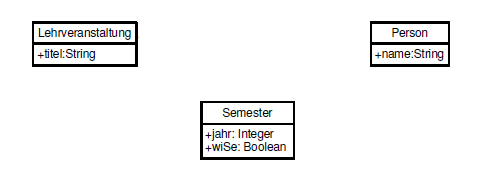
\includegraphics{Objektdiagramm}
\newline
Beim ersten Diagramm besteht diese Beziehung weiterhin auch als einzige einfache Assoziation in der Modellierung, die Klasse \emph{Semester} ist hierbei nämlich als Assoziationsklasse an die Beziehung \emph{nimmt teil an} angegliedert, weitere Assoziationen bestehen in der Darstellung nicht. Diese Form der Modellierung einer mehrstelligen Assoziation ist dann praktisch, wenn gewünscht wird, eine Beziehung mit Attributen zu versehen und damit eine Beziehung zu beschreiben, welche gleichzeitig die Funktion einer Klasse einnimmt, um so die Klassen \emph{Person} und \emph{Lehrveranstaltung} in eine spezifischere Beziehung zu setzen.\newline
Ein Beispiel für diese Umsetzung ließe sich folgendermaßen gestalten:
\newline
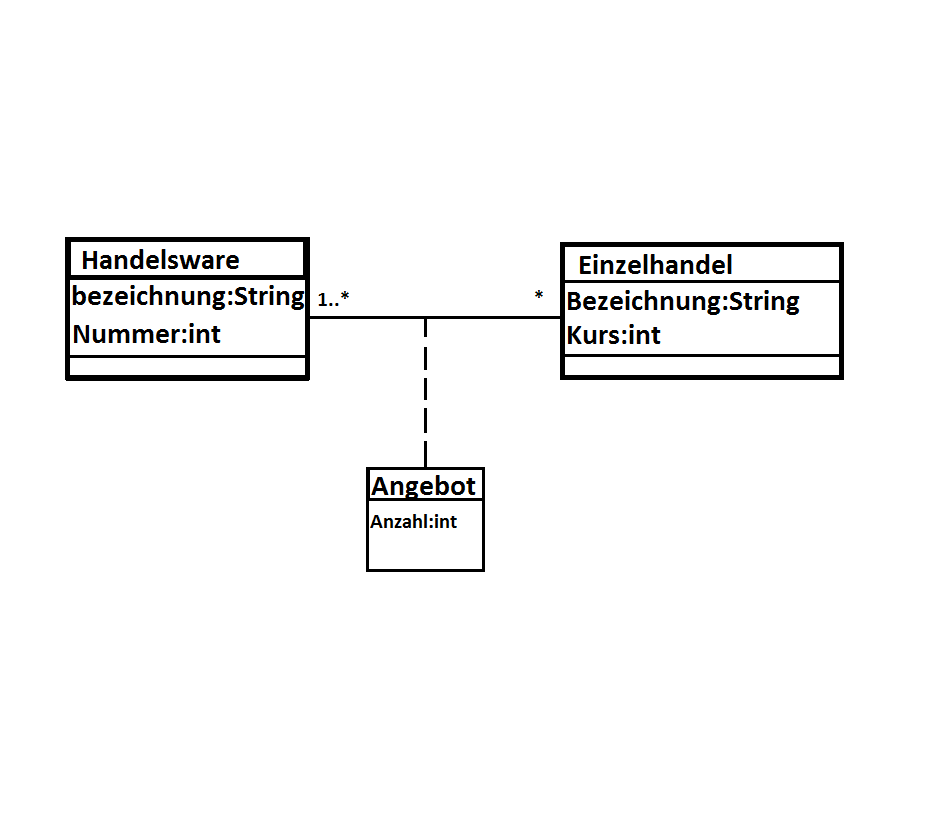
\includegraphics[scale=0.5]{Assoziationsklasse}
\newline
Somit werden in dieser Modellierung die Attribute von \emph{Semester} direkt der Assoziation \emph{nimmt teil an} zugeordnet, was einerseits die Übersichtlichkeit in der Darstellung erhöht, vor allem aber das Abrufen der Attribute im Rahmen der Assoziation ermöglicht, statt eine neue Assoziation zur Klasse \emph{Semester} anlegen und abrufen zu müssen.\newline
\newline
Das zweite Diagramm gestaltet sich in dieser Hinsicht anders, da es auf eine Assoziationsklasse verzichtet und stattdessen die Klasse \emph{Semester} als separate Klasse realisiert, welche in ihre Richtung navigierbare Assoziationen zwischen ihr und der Klasse \emph{Lehrveranstaltung}, in Form der Assoziation \emph{findet statt in}, und der Klasse \emph{Person}, über die Assoziation \emph{nimmt teil in} aufweist.\newline
Diese Darstellung bettet die Attribute der Klasse \emph{Semester} nicht in den Rahmen einer Assoziation ein, sondern verknüpft sie mit den beiden anderen Klassen über jeweils eine gesonderte Assoziation, einer Modellierung, welche sich im Ausbau auch als Realisierung einer mehrstelligen Assoziation durch den Einsatz einer verbindenden Klassen anwenden lässt. Dieser eher klassische Ansatz erlaubt es dann nach folgendem Beispiel mehrere Klassen zugleich miteinander zu assoziieren.\newline
\newline
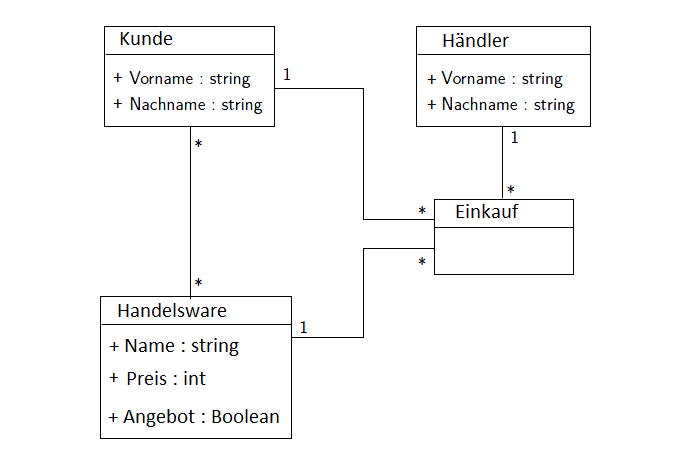
\includegraphics[scale=0.5]{Mehrteilige_Assoziation}
\newline
Konkret unterscheidet sich diese Darstellungsform dahingehend, als dass die Attribute von \emph{Semester} eben nicht nur einer Assoziation zugeordnet werden, sondern über separate Beziehungen abgerufen werden können, was je nach Interessenlage gefragt sein kann.\newline

\textbf{b)}\newline

Gehen wir von der Annahme aus, dass die Attribuierung von \emph{Semester} im Rahmen der Assoziation \emph{nimmt teil an} gefragt ist, so würden wir uns definitiv für die erste Modellierungsvariante entscheiden, da diese eine klare Zuordnung jener Klasse zur Beziehung selbst kennzeichnet. Auf diese Weise ist in übersichtlicher Weise dargestellt, dass im Rahmen der eigentlichen Beziehung der Teilnahme bereits ein Mechanismus zum Abrufen der Attribute zu implementieren ist.\newline
Da auch eine Assoziationsklasse noch mit weiteren Klassen assoziiert werden kann, ist hier auch noch eine weitere Verknüpfung möglich, falls der gesamte Fall ausgebaut werden muss, auch wenn hier die Realisierung als mehrstellige Assoziation über eine Klasse übersichtlicher sein könnte.

\section*{Aufgabe 6)}

Das vorliegende Klassendiagramm weist mehrere Mängel auf. So sind die Multiplizitäten der einzelnen Assoziationen nicht angegeben, wodurch die Standardmultiplizität 1 bei einer Verbindung zu vielen Objekten, wie bei der Klasse \emph{Gruppe} irreführend ist. Ebenso sind die Assoziationen nicht benannt und weisen keine definierten Rollen auf, auch ließe sich die Aggregation zwischen \emph{TutorIn} und \emph{Lehrkraft} anders modellieren sowie Irreführung zu vermeiden und zuletzt sollten Attribute in der Regel versteckt werden, statt in Klassendiagrammen zu Entwurf oder Implementierung öffentlich sichtbar zu sein.

\section*{Aufgabe 7)}

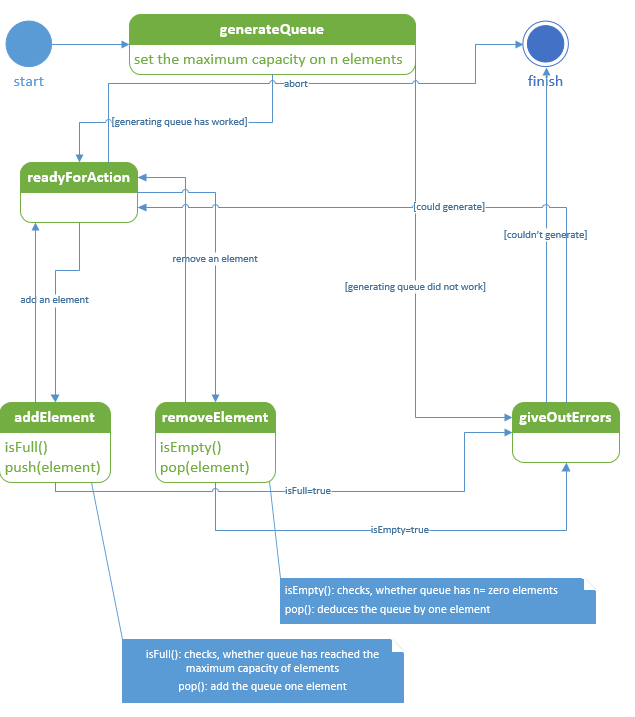
\includegraphics{queue_paint}


\end{document}

